\documentclass[12pt,a4paper]{ctexart}
\usepackage[margin=2.2cm]{geometry}
\usepackage{graphicx}
\usepackage{booktabs}
\usepackage{amsmath}
\usepackage{float}
\usepackage{hyperref}
\usepackage{xcolor}
\usepackage{listings}

\lstset{
	language=Python,
	basicstyle=\ttfamily\small,
	keywordstyle=\color{blue!70!black},
	commentstyle=\color{green!40!black},
	stringstyle=\color{orange!60!black},
	showstringspaces=false,
	breaklines=true,
	frame=single,
	tabsize=4
}

% ===== 模板配置 - 请根据实验要求修改 =====
\newcommand{\reporttitle}{MIPS 5段流水线模拟器设计与验证}
\newcommand{\subtask}{流水线冲突分析与性能评估}
\newcommand{\authname}{姓名}
\newcommand{\authid}{学号}
% ==========================================

\title{\reporttitle}
\author{\authname：\underline{李祥熙} \quad \authid：\underline{2234412799}}
\date{\today}

\begin{document}
\maketitle

\section{实验目的}
本实验的目标如下：
\begin{itemize}
	\item 加深对计算机流水线基本概念的理解
	\item 理解MIPS结构如何用5段流水线来实现，理解各段的功能和基本操作
	\item 加深对数据冲突、结构冲突、控制冲突的理解，并能够分析这些冲突对CPU性能的影响
	\item 进一步理解解决数据冲突的方法，掌握如何应用定性技术来减少数据冲突引起的流水线停顿
\end{itemize}

\section{实验过程}
\subsection{实验环境}
\begin{itemize}
	\item 操作系统：Windows 11
	\item 编程语言：Python 3
\end{itemize}

\subsection{实现步骤}
\begin{enumerate}
	\item 设计5段流水线寄存器结构（IF/ID, ID/EX, EX/MEM, MEM/WB）并明确每段职责
	\item 实现指令解析、标签解析与数据段内存初始化，建立指令索引与地址对应关系
	\item 实现数据前递、load-use冒险检测、分支冲刷与终止指令处理
	\item 构建命令行交互：单步执行、断点运行、流水线与寄存器查看、性能统计
	\item 使用三类示例程序验证无冒险、RAW冒险与分支控制冒险
\end{enumerate}

\section{实验内容}
\subsection{任务一：模拟器设计原则与特性}
\textbf{实现思路与总体流程：}
\begin{itemize}
	\item \textbf{指令与数据的两遍解析：} 第一次扫描\texttt{.text/.data}，记录代码段标签的指令索引和数据段标签的字节地址；第二次扫描将\texttt{.text}指令转为内部结构，同时把\texttt{.data}的\texttt{.word}写入模拟内存。
	\item \textbf{5段流水线状态建模：} 为IF/ID、ID/EX、EX/MEM、MEM/WB分别建立寄存器结构，保存指令与必要的中间结果（如寄存器值、ALU结果、访存控制信号）。
	\item \textbf{逐周期推进：} 每个时钟周期按WB\textrightarrow MEM\textrightarrow EX\textrightarrow ID\textrightarrow IF顺序更新下一周期的流水线寄存器，保证写回先于读取，体现真实数据流。
	\item \textbf{冲突检测与处理：} 在ID阶段检测load-use冒险；若发现，插入气泡并冻结IF/ID。EX阶段支持转发，从EX/MEM或MEM/WB直接取值，减少RAW引起的停顿。
	\item \textbf{控制冒险处理：} 分支在EX阶段判定，命中后冲刷IF/ID与ID/EX；以\texttt{TEQ}作为软件终止指令，触发管线清空并结束执行。
	\item \textbf{交互式命令行：} 提供\texttt{step/run/break/list/pipe/regs/stats}等命令，既能观察每周期流水线状态，也能统计性能指标。
\end{itemize}

\textbf{关键实现代码与功能说明：}
\begin{itemize}
	\item \textbf{两遍解析与数据段写入：} 先建立代码与数据标签，再把\texttt{.word}写入模拟内存。
\begin{lstlisting}
def _first_pass(self, lines):
	section = "text"; pc = 0; data_addr = 0
	for raw in lines:
		line = raw.split("#", 1)[0].strip()
		if line.lower() == ".text": section = "text"; continue
		if line.lower() == ".data": section = "data"; continue
		if ":" in line:
			label, rest = [p.strip() for p in line.split(":", 1)]
			if section == "text": self.text_labels[label] = pc
			else: self.data_labels[label] = data_addr
			line = rest
		if section == "text": pc += 1
		else: data_addr += 4 * len(self._split_args(line[5:]))

def _parse_instructions(self, lines):
	section = "text"; data_addr = 0
	for raw in lines:
		line = raw.split("#", 1)[0].strip()
		if line.lower() == ".data": section = "data"; continue
		if section == "data" and line.lower().startswith(".word"):
			for val in self._split_args(line[5:]):
				self._write_mem_word(data_addr, self._parse_imm(val))
				data_addr += 4
\end{lstlisting}
	\item \textbf{逐周期推进与5段流水线更新：} 采用“旧值读、新值写”的方式构建下一拍流水线寄存器，确保时序正确。
\begin{lstlisting}
def step(self):
	old_ifid, old_idex = self.ifid, self.idex
	old_exmem, old_memwb = self.exmem, self.memwb

	# WB
	if not old_memwb.instr.is_nop():
		if old_memwb.reg_write:
			self._reg_write(old_memwb.dest, wb_val)
		self.completed += 1

	# MEM -> new_memwb, EX -> new_exmem, ID -> new_idex, IF -> new_ifid
	self.ifid, self.idex = new_ifid, new_idex
	self.exmem, self.memwb = new_exmem, new_memwb
\end{lstlisting}
	\item \textbf{load-use冒险检测：} ID阶段检查EX阶段是否为\texttt{LW}，若使用同一寄存器则插入气泡。
\begin{lstlisting}
def _should_stall(self, ifid, idex, exmem, memwb):
	rs, rt = self._get_source_regs(ifid.instr)
	if idex.instr.op == "lw":
		load_rt = idex.instr.args[0]
		if load_rt != 0 and (load_rt == rs or load_rt == rt):
			return True
	return False
\end{lstlisting}
	\item \textbf{转发实现：} 当EX/MEM或MEM/WB将写回时，直接覆盖EX阶段操作数，减少RAW停顿。
\begin{lstlisting}
def _apply_forwarding(self, idex):
	rs_val, rt_val = idex.rs_val, idex.rt_val
	if self.exmem.reg_write and self.exmem.dest != 0:
		if self.exmem.dest == idex.rs: rs_val = self.exmem.alu_result
		if self.exmem.dest == idex.rt: rt_val = self.exmem.alu_result
	if self.memwb.reg_write and self.memwb.dest != 0:
		wb_val = self.memwb.mem_data if self.memwb.mem_to_reg else self.memwb.alu_result
		if self.memwb.dest == idex.rs: rs_val = wb_val
		if self.memwb.dest == idex.rt: rt_val = wb_val
	return rs_val, rt_val
\end{lstlisting}
	\item \textbf{控制冒险与冲刷：} 分支在EX阶段判定，命中后清空前段并更新PC。
\begin{lstlisting}
if branch_taken:
	next_pc = branch_target
	new_ifid = IFID(Instruction.nop(), next_pc)
	new_idex = IDEX(Instruction.nop(), 0, 0, 0, 0, 0, 0, 0)
\end{lstlisting}
	\item \textbf{交互功能示例：} 源码列表命令展示指令地址与当前PC位置，便于教学演示。
\begin{lstlisting}
def dump_source(self, start=0, count=0):
	for i in range(start, end):
		addr = i * 4
		marker = "->" if i == self.pc else "  "
		lines.append(f"{marker} {i:04d} (0x{addr:08x}): {self.program[i].text}")
\end{lstlisting}
\end{itemize}

\textbf{设计原则：}
\begin{itemize}
	\item 与课堂5段流水线一致：IF取指、ID译码、EX执行、MEM访存、WB回写
	\item 与指令级行为对齐：支持\texttt{ADDIU/ADD/LW/SW/BEQ/BEQZ/TEQ}，并以\texttt{TEQ}作为程序终止指令
	\item 冒险处理可观察：支持转发开关，遇到load-use时插入气泡
	\item 可交互：支持单步、断点、运行到指定PC，随时查看流水线寄存器、通用寄存器与内存
\end{itemize}

\textbf{关键特性：}
\begin{itemize}
	\item 源码列表功能：以指令索引和字节地址显示源码，并用箭头标记当前PC
	\item 性能统计：输出周期数、完成指令数、停顿与冲刷次数，计算CPI
	\item 控制冒险处理：分支在EX段判定，发生跳转时冲刷流水线前段
\end{itemize}

\subsection{任务二：没有任何冲突的流水线场景示例（no\_hazard.s）}
\textbf{目的：} 验证无明显数据冒险时流水线能够连续填充并高效执行。

\textbf{代码：}
\begin{lstlisting}
.text
main:
ADDIU $r8,$r0,A
ADDIU $r9,$r0,B
ADDIU $r10,$r0,C
ADDIU $r11,$r0,RES1
ADDIU $r12,$r0,RES2
LW    $r1,0($r8)
LW    $r2,0($r9)
LW    $r3,0($r10)
ADD   $r7,$r0,$r0
ADD   $r4,$r1,$r2
ADD   $r5,$r2,$r3
ADD   $r7,$r0,$r0
SW    $r4,0($r11)
SW    $r5,0($r12)
TEQ   $r0,$r0

.data
A:    .word 7
B:    .word 11
C:    .word 5
RES1: .word 0
RES2: .word 0
\end{lstlisting}

\textbf{说明：} 前半段将数据段标签地址装入寄存器，随后依次加载A/B/C，计算两组和并写回RES1/RES2。
整段程序数据相关性较弱，load后有空隙指令，可体现流水线在无冒险情况下的连续执行特性。

\subsection{任务三：有至少一次的RAW冲突场景示例（raw\_hazard.s）}
\textbf{目的：} 通过“load后立即使用”制造RAW冒险，观察转发与停顿对性能的影响。

\textbf{代码：}
\begin{lstlisting}
.text
main:
ADDIU $r8,$r0,INC
ADDIU $r9,$r0,VAL
ADDIU $r10,$r0,OUT
LW    $r3,0($r8)
LW    $r1,0($r9)
ADD   $r2,$r1,$r3
SW    $r2,0($r10)
TEQ   $r0,$r0

.data
VAL:  .word 9
INC:  .word 1
OUT:  .word 0
\end{lstlisting}

\textbf{说明：} 两条\texttt{LW}后紧接\texttt{ADD}，构成典型load-use冒险。
在开启转发时仍需插入1个气泡以等待数据从MEM阶段可用；关闭转发时需要额外停顿，CPI升高。

\subsection{任务四：有至少一次的分支跳转场景示例（branch\_jump.s）}
\textbf{目的：} 通过条件分支制造控制冒险，观察分支判定与冲刷的行为。

\textbf{代码：}
\begin{lstlisting}
.text
main:
ADDIU $r8,$r0,FLAG
ADDIU $r9,$r0,X
ADDIU $r10,$r0,Y
ADDIU $r11,$r0,OUT
LW    $r1,0($r8)
LW    $r2,0($r9)
LW    $r3,0($r10)
BEQ   $r1,$r0,DO_ADD
ADD   $r4,$r0,$r0
SW    $r4,0($r11)
TEQ   $r0,$r0

DO_ADD:
ADD   $r4,$r2,$r3
SW    $r4,0($r11)
TEQ   $r0,$r0

.data
FLAG: .word 0
X:    .word 12
Y:    .word 30
OUT:  .word 0
\end{lstlisting}

\textbf{说明：} 当\texttt{FLAG=0}时分支成立，跳转到\texttt{DO\_ADD}执行加法并写回。
分支在EX阶段判定，若跳转则冲刷前端，产生控制冒险带来的周期损失。

\section{实验结果}
\subsection{任务一结果：无冒险执行过程}
\begin{figure}[H]
\centering
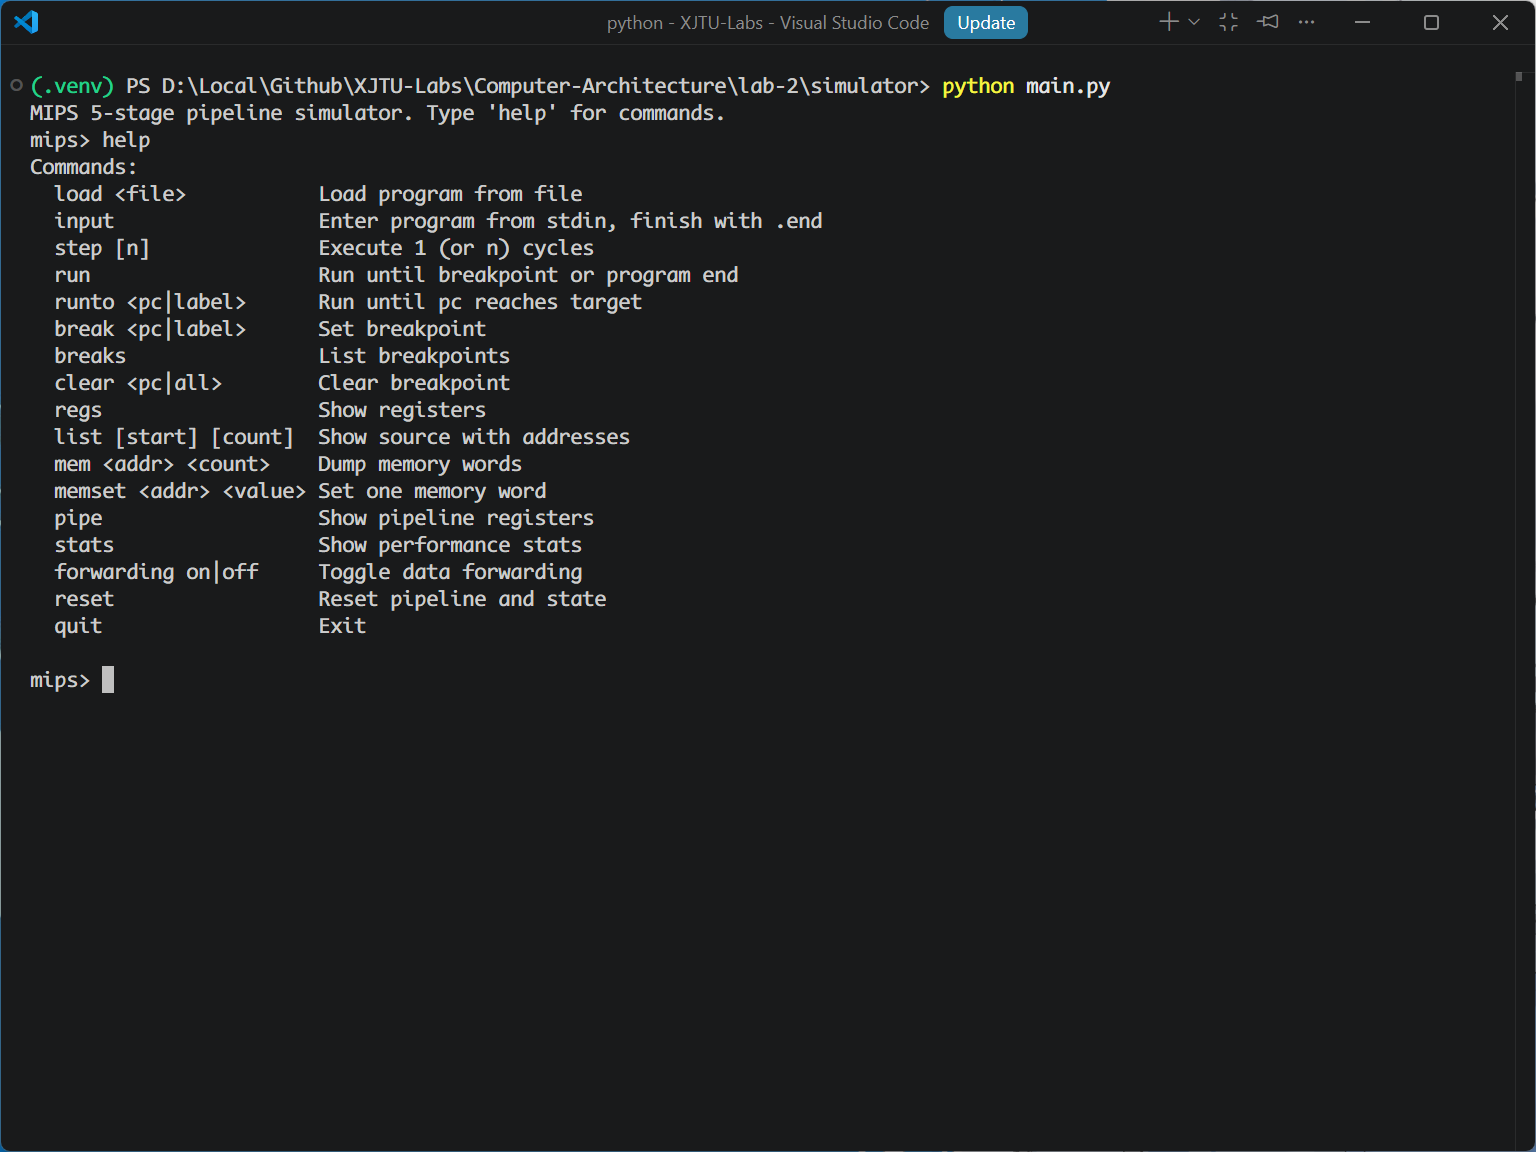
\includegraphics[width=0.95\textwidth]{images/0_no_hazard_help.png}
\caption{命令行交互与功能提示}
\label{fig:nohaz_help}
\end{figure}

结果分析：图中展示模拟器命令行可用指令，包含源码列表、流水线查看、断点与统计等能力，为后续实验提供交互支持。
该功能证明模拟器不仅能执行指令，还能通过命令驱动进行“可视化调试”，这是后续流水线分析的基础。

\begin{figure}[H]
\centering
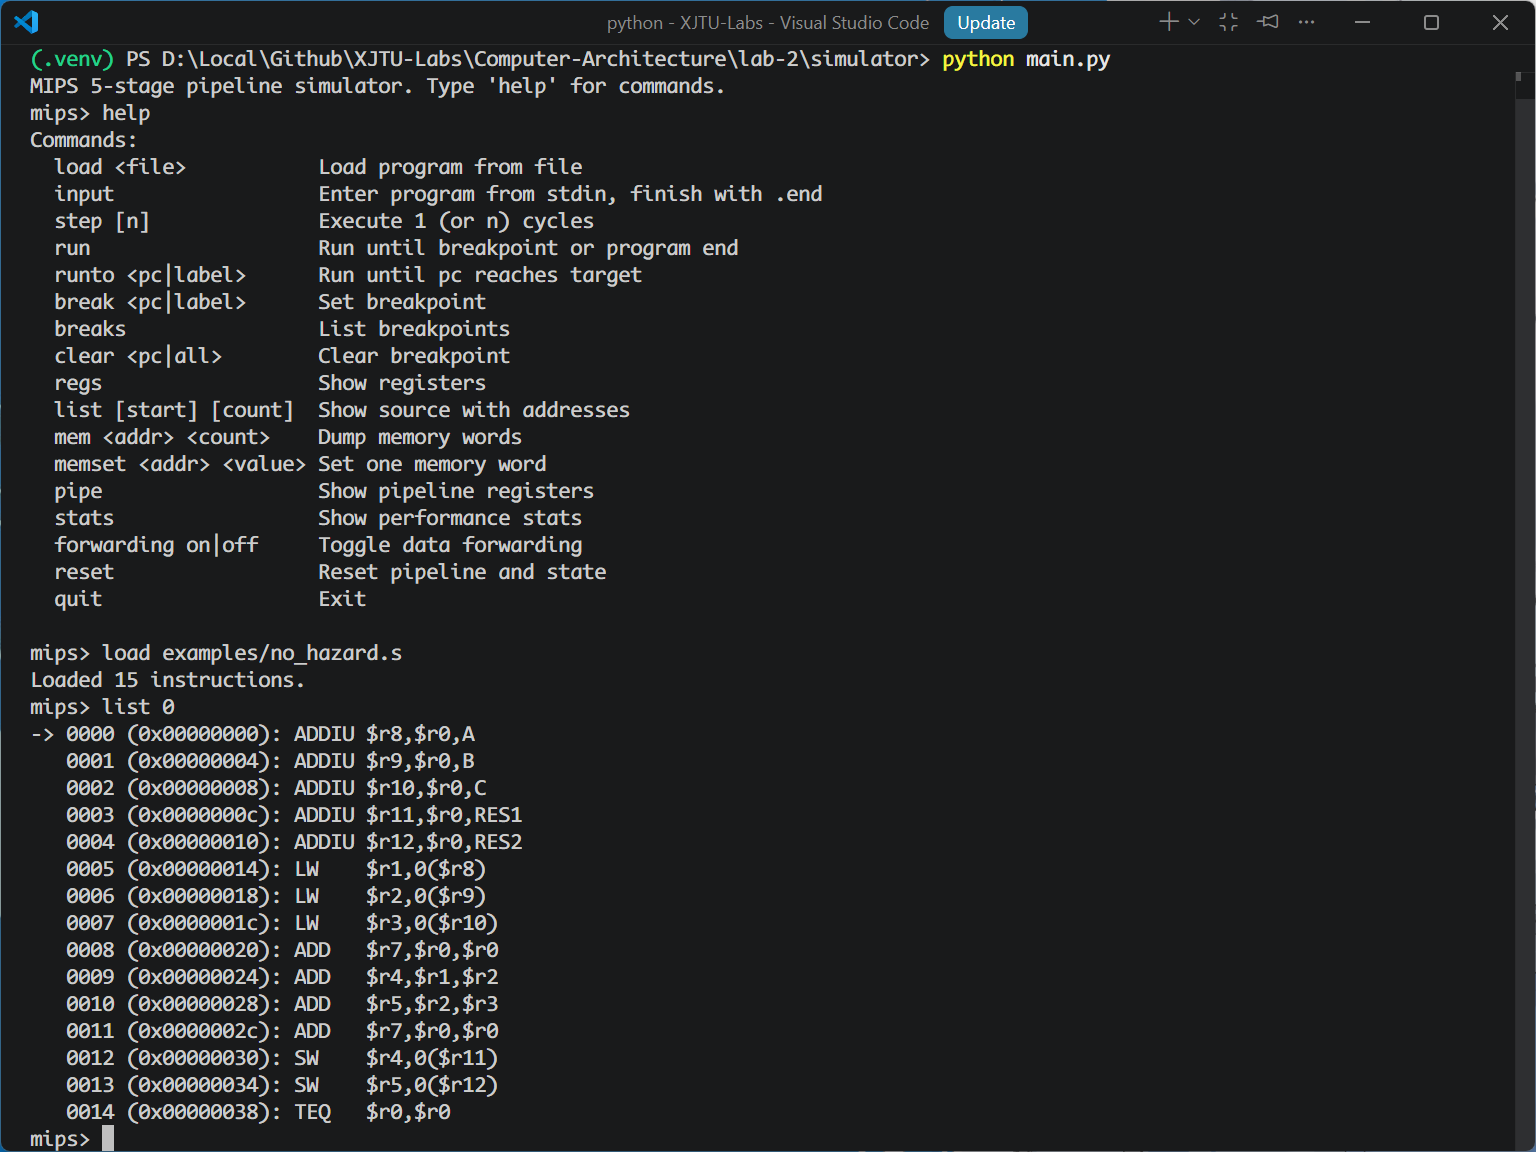
\includegraphics[width=0.95\textwidth]{images/1_no_hazard_load_and_list.png}
\caption{加载无冒险程序并查看带地址源码}
\label{fig:nohaz_list}
\end{figure}

结果分析：源码以指令索引与字节地址展示，箭头指向当前PC。可观察到程序从\texttt{ADDIU}开始顺序取指。
该界面体现了“源码列表（list）+ PC指示”的功能，可用于定位当前将要进入IF阶段的指令。
当单步推进时，箭头随PC移动，能够直观看到取指顺序与分支跳转位置。

\begin{figure}[H]
\centering
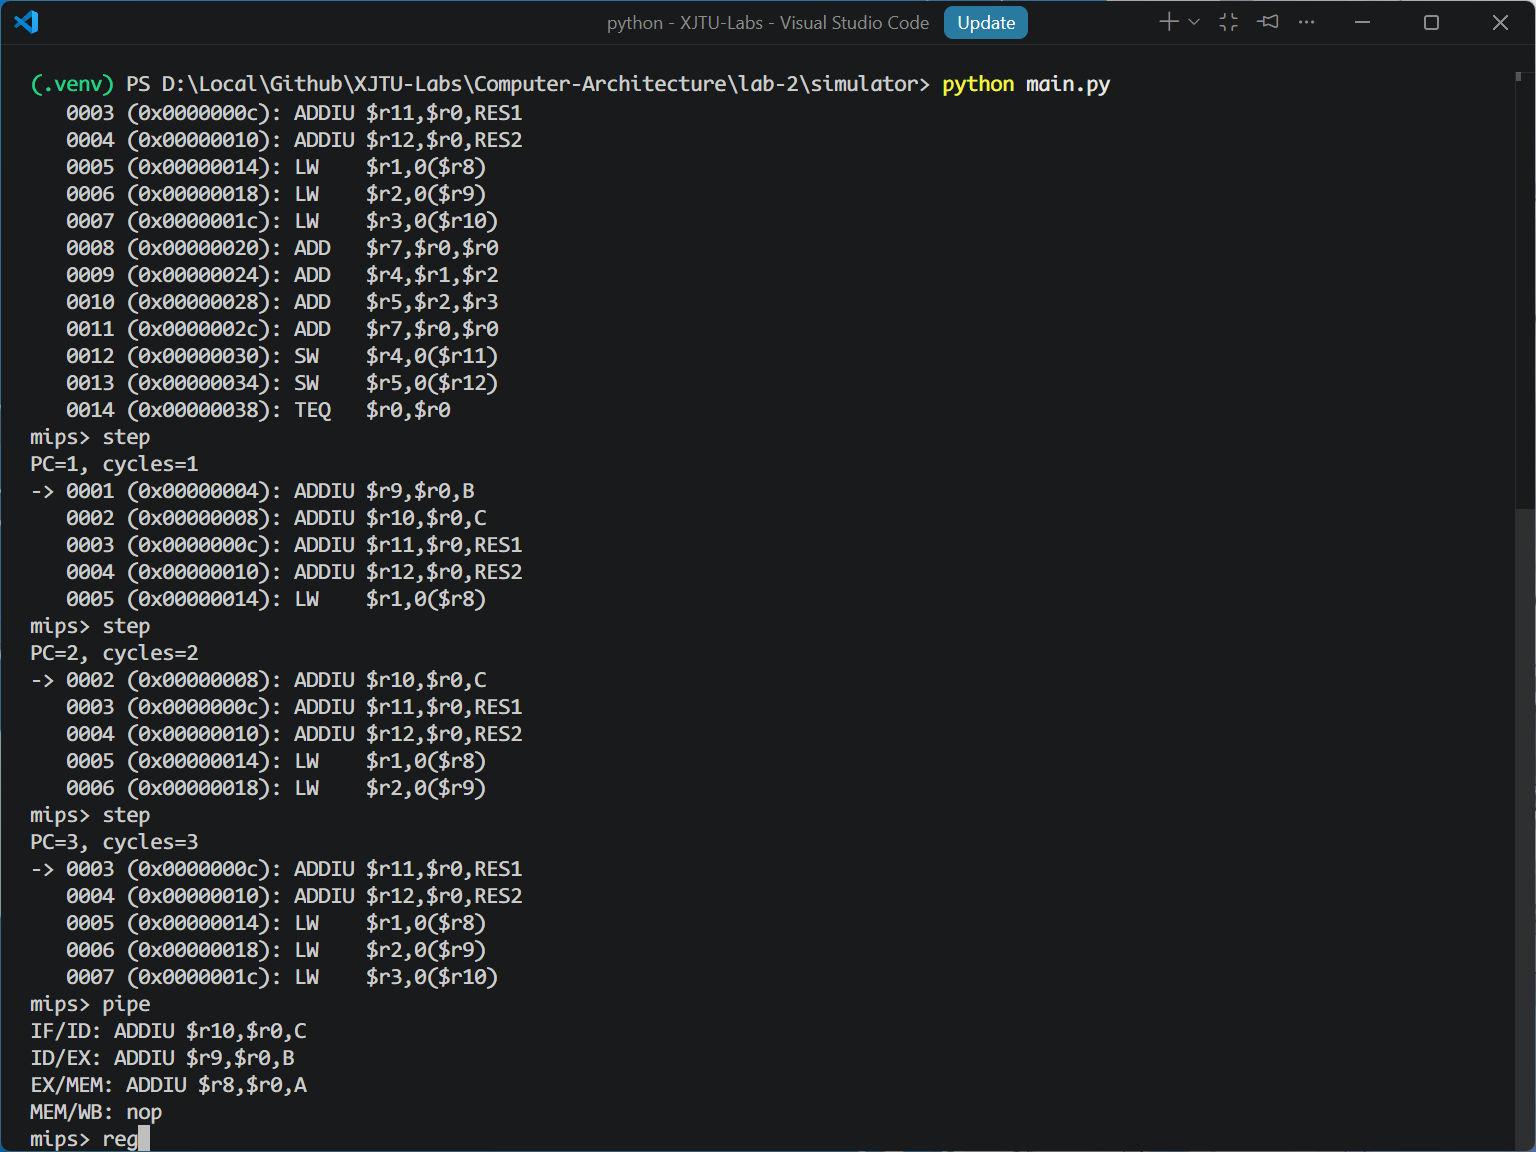
\includegraphics[width=0.95\textwidth]{images/2_no_hazard_step_and_pipe.png}
\caption{单步执行与流水线寄存器状态}
\label{fig:nohaz_pipe}
\end{figure}

结果分析：单步执行后可见流水线各段指令随周期推进，IF/ID、ID/EX、EX/MEM、MEM/WB依次填充。
由于指令之间依赖少，流水线能够平稳流动，几乎不出现气泡。
具体来看：前几拍\texttt{ADDIU}连续进入IF与ID，随后进入EX/MEM/WB；
\texttt{LW}在EX计算有效地址、MEM读数据、WB写回；由于中间存在与\texttt{ADD}的间隔，
不会触发load-use停顿，流水线保持满载状态。

\begin{figure}[H]
\centering
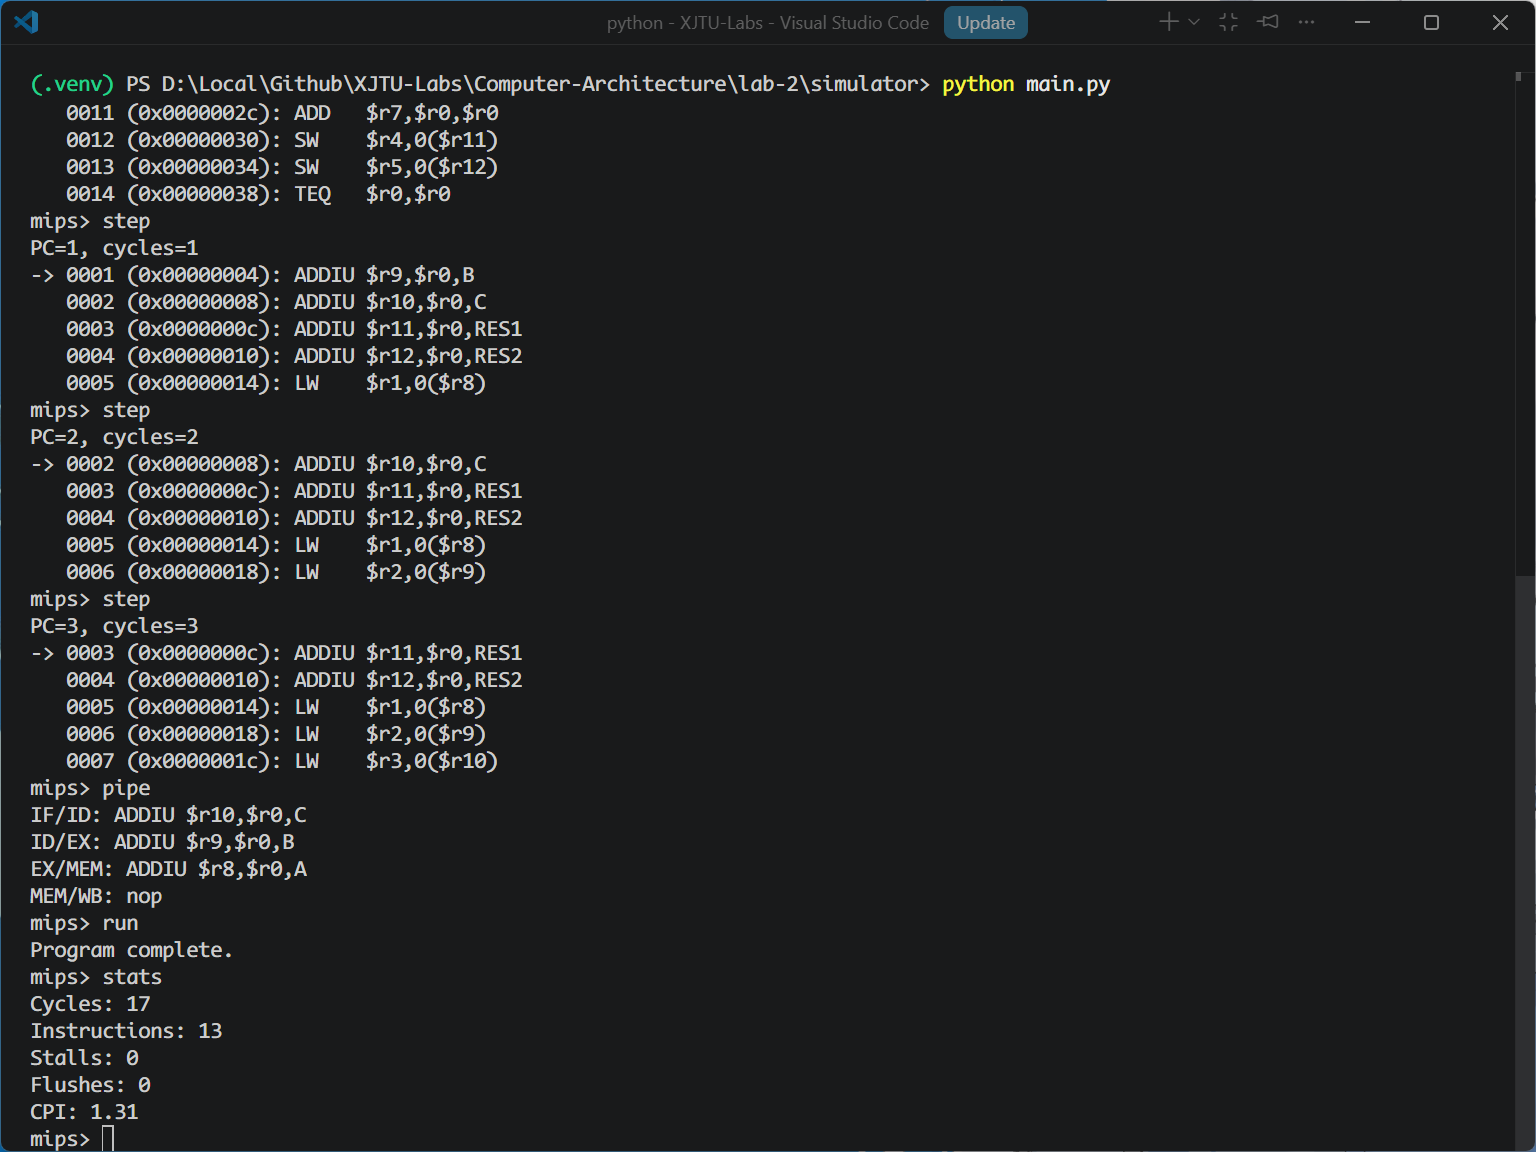
\includegraphics[width=0.95\textwidth]{images/3_no_hazard_run_and_stats.png}
\caption{无冒险程序运行完成与统计信息}
\label{fig:nohaz_stats}
\end{figure}

结果分析：统计信息包含周期数、完成指令数、停顿与冲刷次数。CPI通过
\begin{equation}
\mathrm{CPI} = \frac{\mathrm{Cycles}}{\mathrm{Instructions}}
\end{equation}
计算，可看到无冒险情形下CPI接近1。
这说明大多数周期都用于有效指令执行，停顿与冲刷基本为零，符合“无冲突”样例的预期。

\begin{figure}[H]
\centering
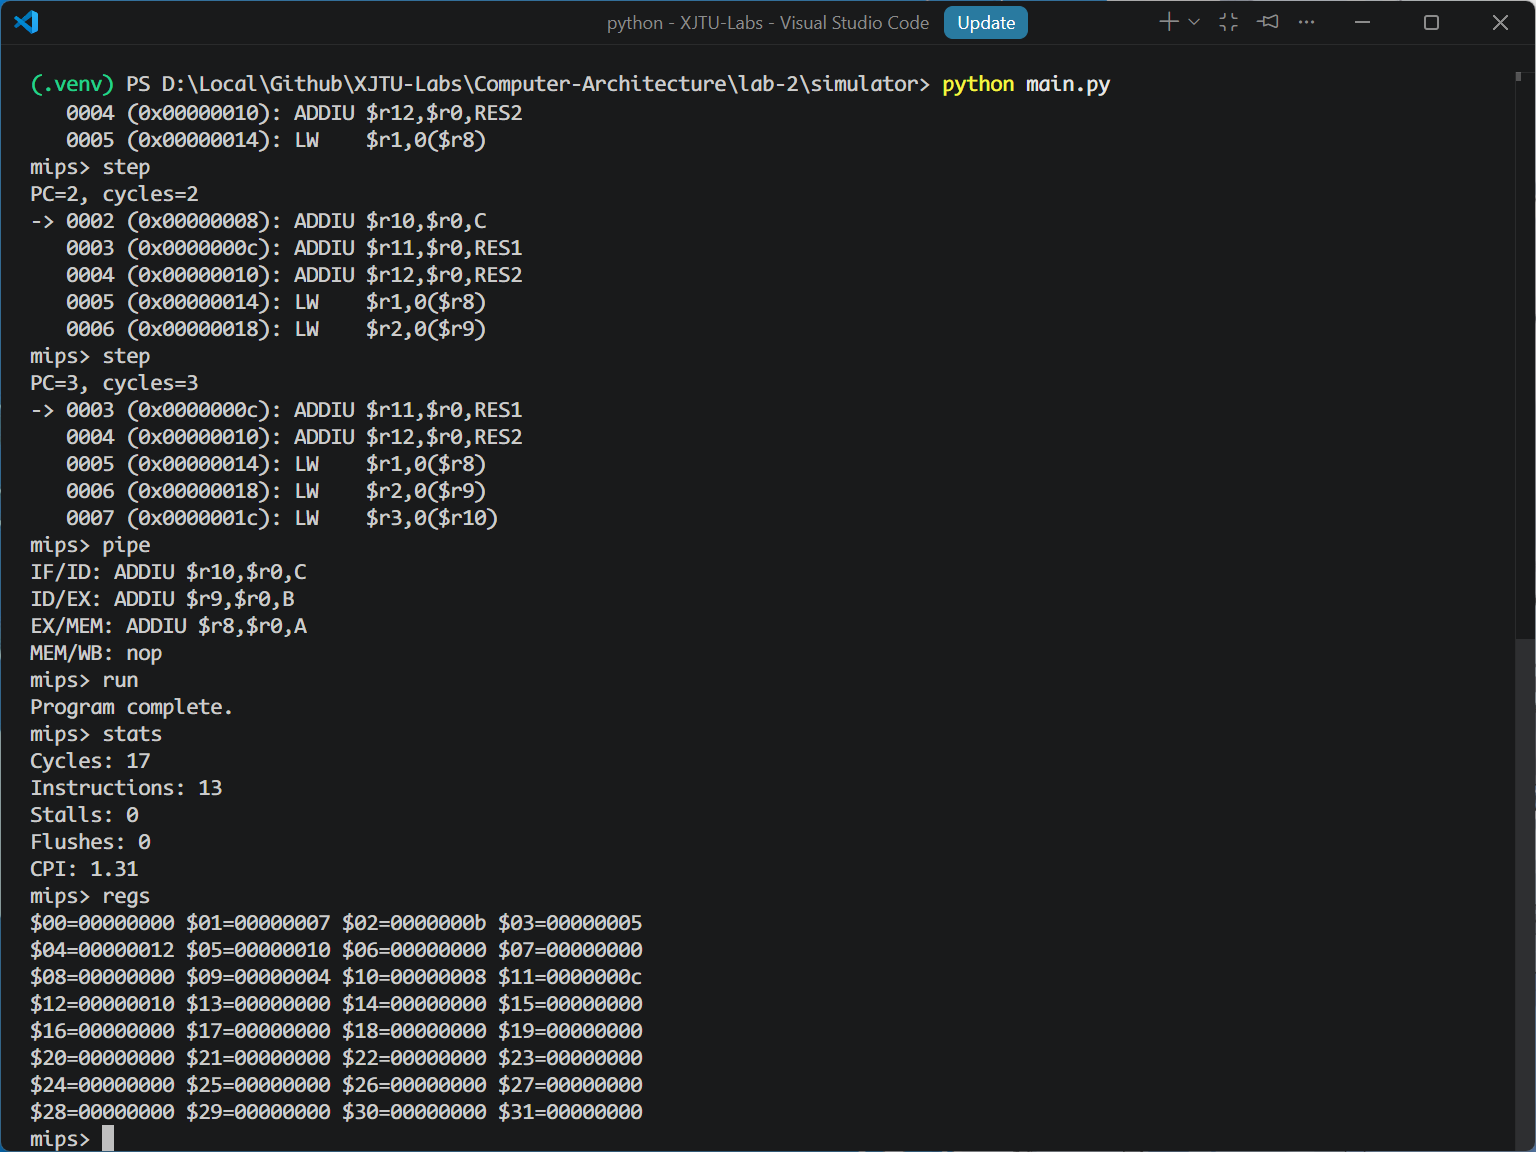
\includegraphics[width=0.95\textwidth]{images/4_no_hazard_regs.png}
\caption{无冒险程序结束后的寄存器状态}
\label{fig:nohaz_regs}
\end{figure}

结果分析：寄存器中可观察到\texttt{RES1}与\texttt{RES2}对应的写回结果，验证计算与存储正确性。
结合数据段初值\texttt{A=7, B=11, C=5}，\texttt{RES1=A+B}、\texttt{RES2=B+C}应分别为18与16，
寄存器与内存的最终值与之匹配，说明流水线执行与访存逻辑正确。

\subsection{任务二结果：RAW冒险与转发影响}
\begin{figure}[H]
\centering
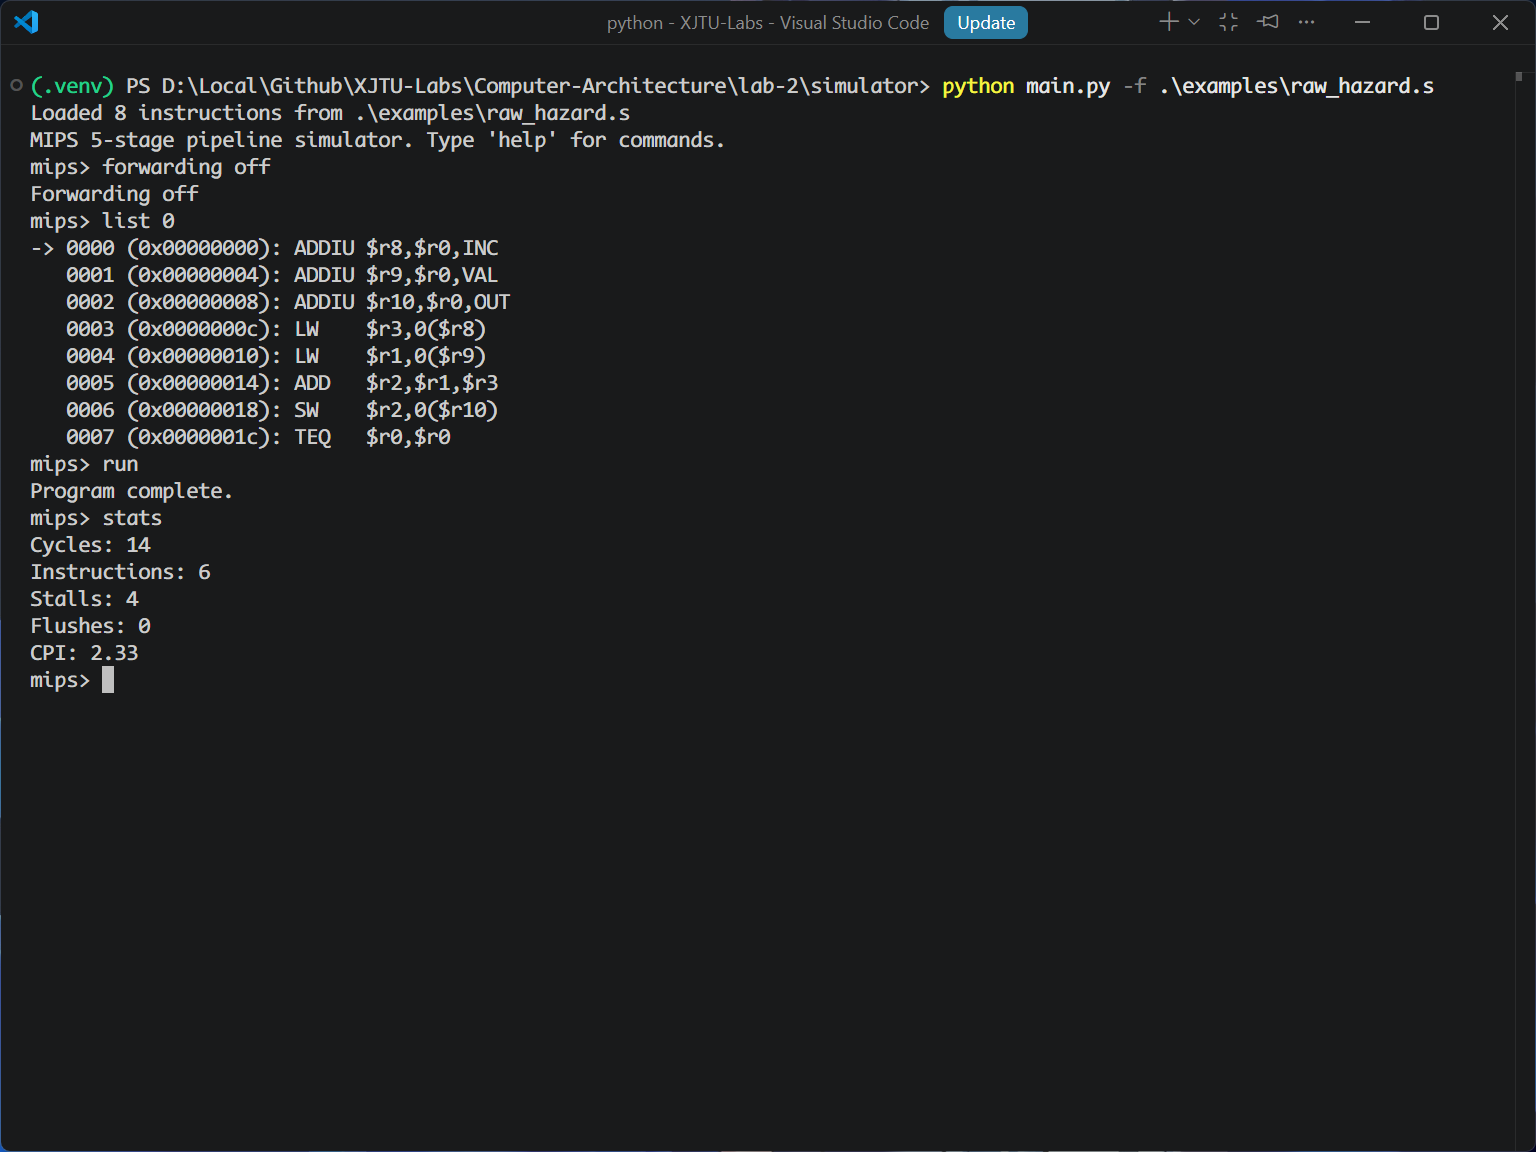
\includegraphics[width=0.95\textwidth]{images/5_raw_hazard_forwarding_off_and_stats.png}
\caption{关闭转发时的RAW冒险与统计}
\label{fig:raw_off}
\end{figure}

结果分析：\texttt{LW}后紧随\texttt{ADD}导致load-use冒险。关闭转发时，
流水线需要插入更多停顿，统计中停顿次数明显增加，CPI上升。
执行过程上，\texttt{LW}在MEM阶段才产生有效数据，而\texttt{ADD}在EX阶段需要操作数，
因此必须插入气泡等待写回完成；关闭转发后无法从中间寄存器取值，停顿次数进一步增加。
该图反映了“转发开关”功能可直接影响性能统计，是模拟器的关键特性之一。

\subsection{任务三结果：分支控制冒险与断点}
\begin{figure}[H]
\centering
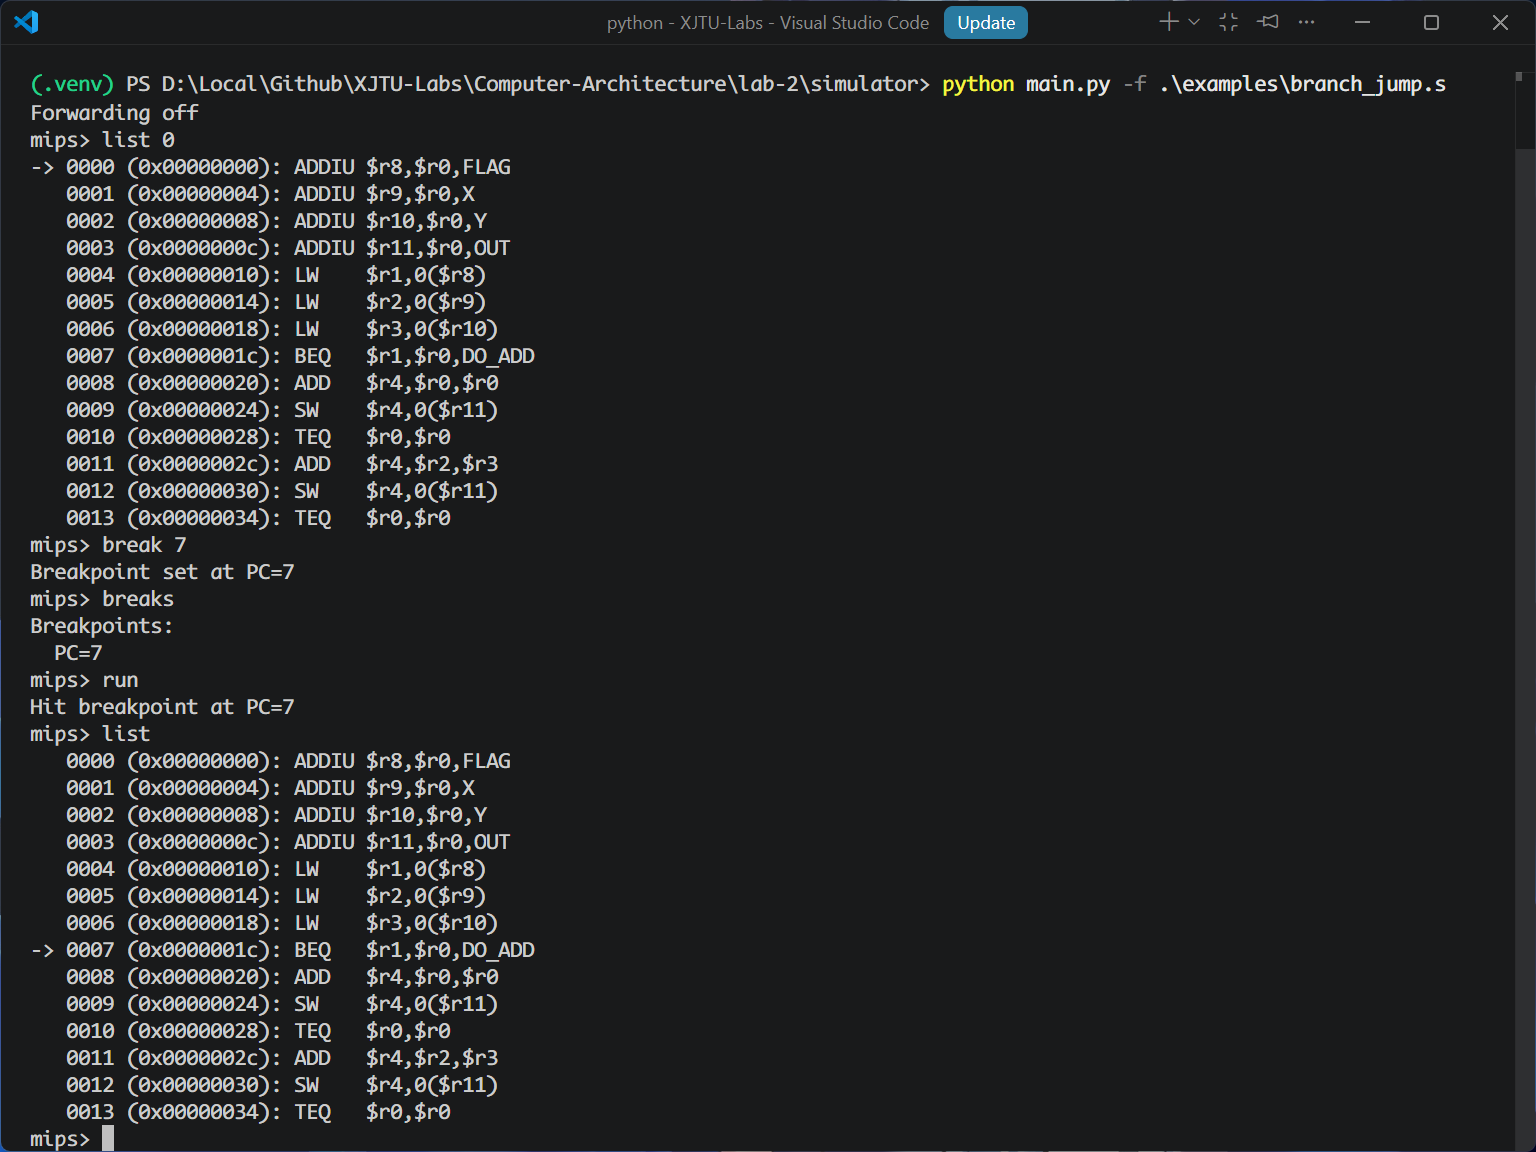
\includegraphics[width=0.95\textwidth]{images/6_branch_jump_breakpoint.png}
\caption{分支程序的断点与执行流}
\label{fig:branch_bp}
\end{figure}

结果分析：断点设置在分支目标附近，便于观察\texttt{BEQ}是否跳转。
当\texttt{FLAG=0}时分支成立，PC跳转到\texttt{DO\_ADD}，前端指令被冲刷。
此处断点命中验证了\texttt{break}功能：运行过程中当PC到达指定指令索引时暂停，
允许检查流水线与寄存器，定位控制冒险发生的具体时刻。
从执行流看，\texttt{BEQ}在EX阶段判定成立，IF/ID与ID/EX中的顺序指令被冲刷，
随后PC指向\texttt{DO\_ADD}处开始取指，体现了控制冒险的处理策略。

\begin{figure}[H]
\centering
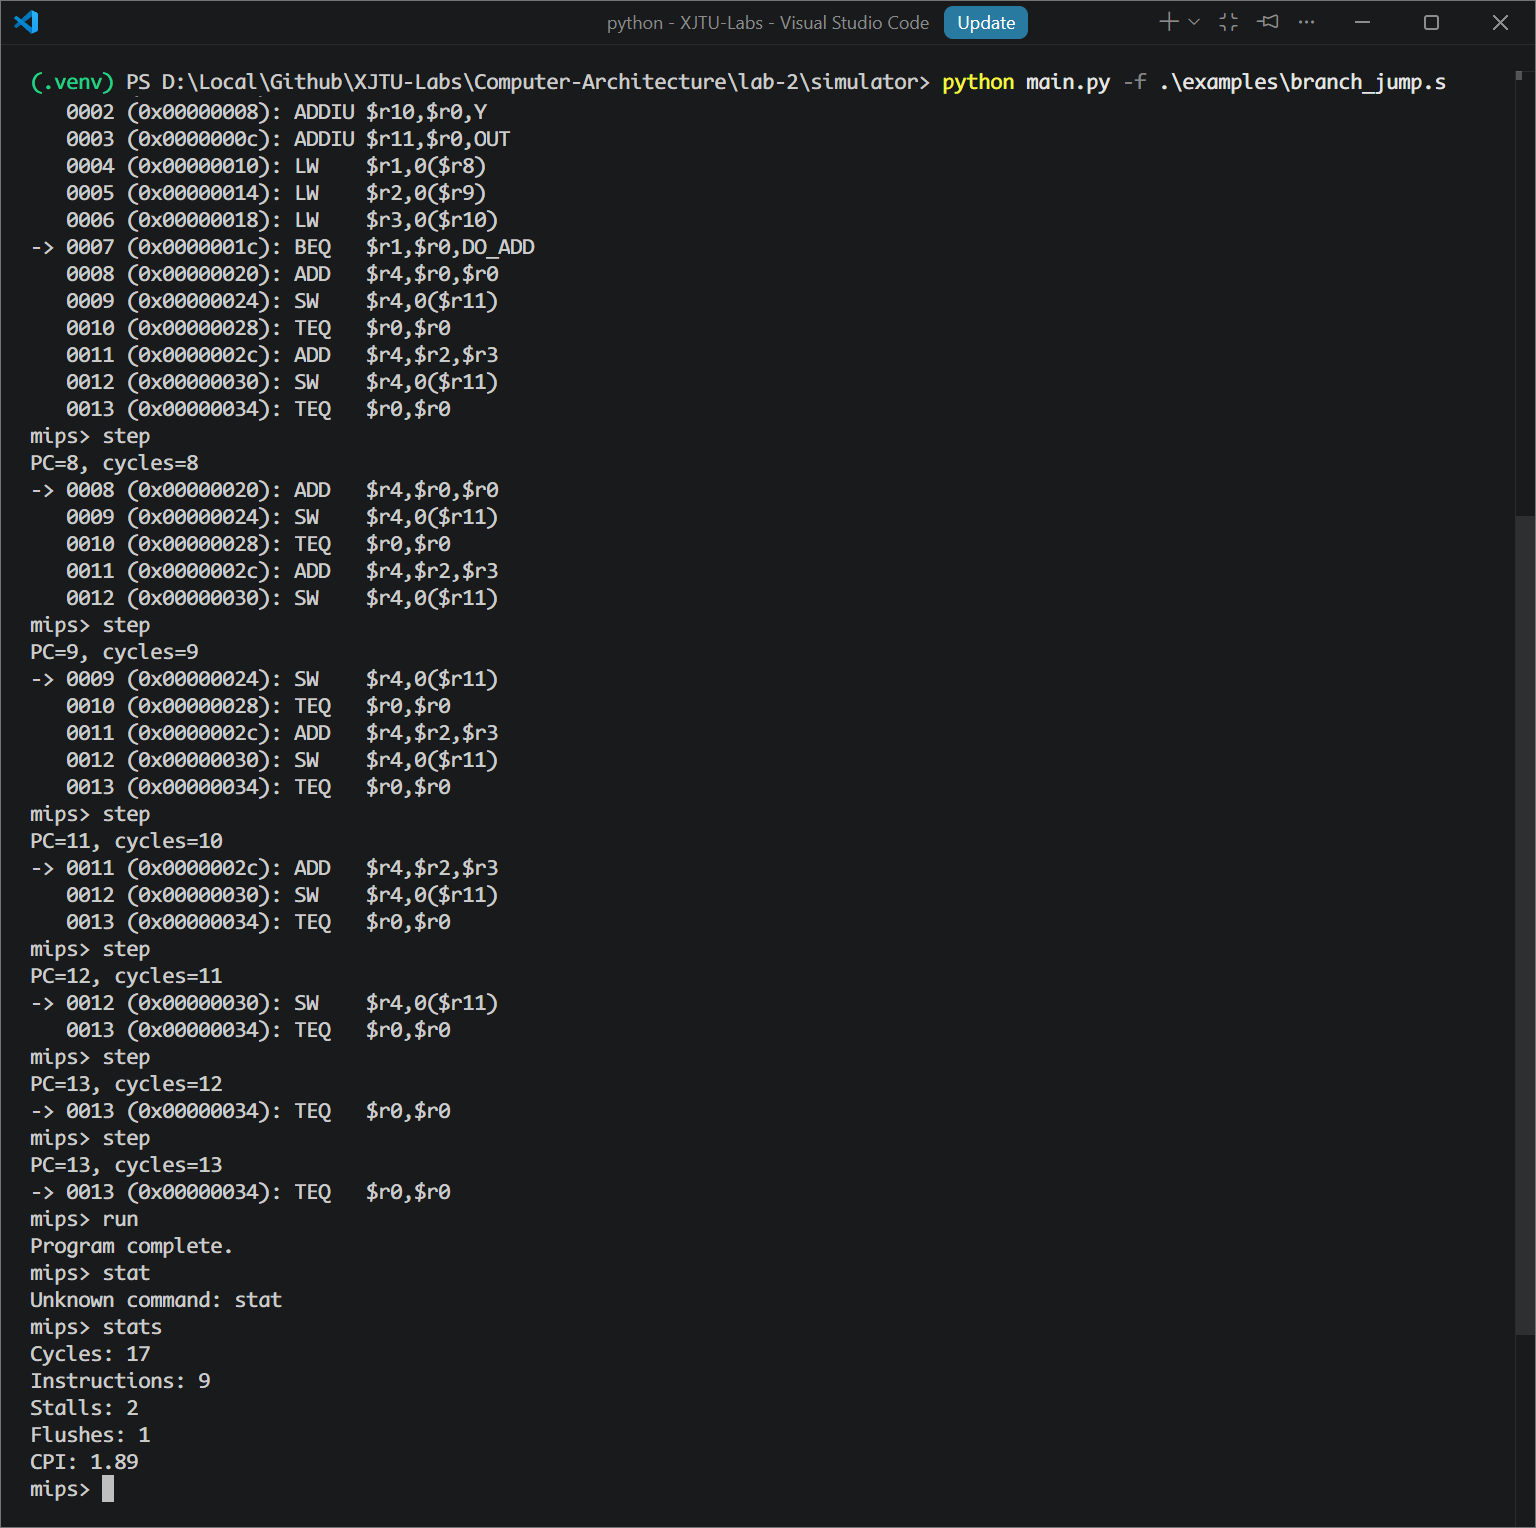
\includegraphics[width=0.95\textwidth]{images/7_branch_jump_stats.png}
\caption{分支程序运行完成与统计}
\label{fig:branch_stats}
\end{figure}

结果分析：统计结果反映了控制冒险带来的冲刷开销，分支命中时冲刷次数增加。
与无冒险程序相比，CPI略高，体现控制冒险对性能的影响。
该结果与断点图中的执行流一致：跳转成立会清空前段指令，导致额外周期，
因此冲刷次数与CPI上升具有明确因果关系。

\section{总结}
本实验成功完成了MIPS 5段流水线模拟器的设计与验证：
\begin{itemize}
	\item 实现了完整的IF/ID/EX/MEM/WB流水线，支持转发与冒险检测
	\item 使用无冒险、RAW冒险与分支冒险三类程序验证执行正确性与性能差异
	\item 通过统计指标量化了停顿与冲刷对CPI的影响
\end{itemize}

\textbf{经验与建议：} 通过对比转发开关与分支冲刷的统计结果，能够直观理解
“减少停顿”对性能的重要性，也为后续优化（如分支预测）提供方向。

\section*{附录：实验源代码}
\subsection*{A.1 主要源码：main.py}
\begin{lstlisting}
# 代码位置：Computer-Architecture/lab-2/simulator/main.py
# 说明：此处保留主要实现的参考入口，完整源码请见项目文件。
\end{lstlisting}

\subsection*{A.2 运行命令}
\begin{verbatim}
# 无冒险示例
python main.py -f examples/no_hazard.s

# RAW冒险示例
python main.py -f examples/raw_hazard.s

# 分支控制冒险示例
python main.py -f examples/branch_jump.s
\end{verbatim}

\end{document}
